\chapter{Model Architecture and Learning Mechanisms}

\section{Overview}

\section{Vision Model}
\textit{TODO: Must say that CNN is used as a visual feature extractor}

The Convolutional Neural Network module used in the models is a variant of well-know AlexNet \cite{NIPS2012_4824}. The network is comprised of eight layers with weights: the first five are convolutional and the last three are fully-connected. There are several pooling and nonlinear layers stacked in-between convolutional layers. The difference between CNN used in this thesis with the original AlexNet lies in the fact that instead of \textit{splitting} the network into two identifical parts (each with halves of the parameters), I use one unified architecture of the network. In addition, normalization layers are omitted as they are proved to be not efficient. Except for the first layer whose input is an image, the output of the previous layer is fed as the input to the next layer. Detailed architecture of the network is explained as follow.

\begin{itemize}
	\item[--] The input to the first convolutional layer  -- namely \texttt{conv1} -- is an image of size $224 \times 224 \times 3$ \footnote{number 3 represents the R-G-B color channels of the image} which is filtered by 96 filters of size $11 \times 11 \times 3$ with stride \footnote{Stride is the distance between the receptive field centers of neighboring neurons in a kernel maps} $S = 4$. The output of \texttt{conv1} is fed into a ReLU layer (\texttt{relu1}) and then max-pooled (\texttt{pool1}) with filter size of 2.

	\item[--] The second convolutional layer  -- \texttt{conv2} -- takes as input the output of \texttt{pool1} and filters it with 256 kernels of size $5 \times 5 \times 48$.

	\item[--] The third convolutional layer -- \texttt{conv3} -- 
\end{itemize}

Altogether, those layers make up (\textit{TODO: use another verb phrase}) a deep convolutional neural network with approximately 60 millions learnable parameters. The details of parameters for each layer is illustrated in table \ref{tab:alexnet-params}

\begin{table}
	\centering
       \label{tab:alexnet-params}
       \begin{tabular}{|l|l|l|c|c|c|c|c|c|r|} \hline
              \textbf{No.} & \textbf{Layer} & \textbf{Type} & \textbf{K} & \textbf{F} & \textbf{S} & \textbf{P} & \textbf{Pool} & \textbf{Output size} & \textbf{Params} \\ \hline
              \multirow{3}{*}{1} & conv1 & convolution & 96 & 11 & 4 & 0 & & $\left[ 55 \times 55 \times 96 \right]$ & 34,848 \\ \cline{2-10}
                          & relu1 & ReLU & & & & & & &  \\ \cline{2-10}
                          & pool1 & pooling & & 3 & 2 & & MAX & $\left[ 27 \times 27 \times 96 \right]$ & \\ \hline
                          % & norm1 & LRN & & & & & & & \\ \hline
              \multirow{3}{*}{2} & conv2 & convolution & 256 & 5 & 1 & 2 & & $\left[ 27 \times 27 \times 256 \right]$ & 614,400\\ \cline{2-10}
                          & relu2 & ReLU & & & & & & &\\ \cline{2-10}
                          & pool2 & pooling & & 3 & 2 & & MAX & $\left[ 13 \times 13 \times 256 \right]$ & \\ \hline
                          % & norm2 & LRN & & & & & & & \\ \hline
              \multirow{3}{*}{3} & conv3 & convolution & 384 & 3 & 1 & 3 & & $\left[ 13 \times 13 \times 384 \right]$ & 884,736 \\ \cline{2-10}
                          & relu3 & ReLU & & & & & & & \\ \hline
              \multirow{2}{*}{4} & conv4 & convolution & 384 & 3 & 1 & 3 & & $\left[ 13 \times 13 \times 384 \right]$ & 663,552\\ \cline{2-10}
                          & relu4 & ReLU & & & & & & & \\ \hline
              \multirow{3}{*}{5} & conv5 & convolution & 256 & 3 & 1 & 1 & & $\left[ 13 \times 13 \times 256 \right]$ & 884,736 \\ \cline{2-10}
                          & relu5 & ReLU & & & & & & & \\ \cline{2-10}
                          & pool5 & pooling & & 3 & 2 & & MAX & $\left[ 6 \times 6 \times 256 \right]$ & \\ \hline 
              \multirow{3}{*}{6} & fc6 & fully-connected & & & & & & $\left[ 1 \times 1 \times 4096 \right]$ & 37,748,736  \\ \cline{2-10}
                          & relu6 & ReLU & & & & & & & \\ \cline{2-10}
                          & dropout6 & dropout (50\%) & & & & & & & \\ \hline
              \multirow{3}{*}{7} & fc7 & fully-connected & & & & & & $\left[ 1 \times 1 \times 4096 \right]$ & 16,777,216 \\ \cline{2-10}
                          & relu7 & ReLU & & & & & & & \\ \cline{2-10}
                          & dropout7 & dropout (50\%) & & & & & & & \\ \hline
              \multirow{2}{*}{8} & fc8 & fully-connected & & & & & & $\left[ 1 \times 1 \times 35 \right]$ & 143,360 \\ \cline{2-10}
                          & loss & SoftMax & & & & & & $\left[ 1 \times 1 \times 35 \right]$ & \\ \hline
       \end{tabular}
       \caption*{AlexNet's architecture details. $K$: the number of filters in a layer; $F:$ size of receptive fields; $S:$ number of stride; $P:$ size of \emph{zero-padding} which pads the input with zeros on the border of input volume}

\end{table}

\section{Language Model}

Long-Short Term Memory (LSTM) \cite{Hochreiter:1997:LSM:1246443.1246450} is used as language model. 

\begin{align}
  i_t &= \sigma \left( W_{ix}x_t + W_{im}m_{t-1}\right) \\
  f_t &= \sigma \left( W_{fx}x_t + W_{fm}m_{t-1}\right) \\
  o_t &= \sigma \left( W_{ox}x_t + W_{om}m_{t-1}\right) \\
  c_t &= f_t \odot c_{t-1} + i_t \odot h\left( W_{cx}x_t + W_{cm}m_{t-1}\right)\\
  m_t &= o_t \odot c_t \\
  p_{t+1} &= \text{Softmax} \left( m_t \right)
\end{align}
\section{Learning Mechanims}
The model is trained using stochastic gradient descent with Adam optimization method \cite{DBLP:journals/corr/KingmaB14}. The training loss is shown in Figure \ref{fig:vgg_adam}

\begin{figure}
  \label{fig:vgg_adam}
  \centering
  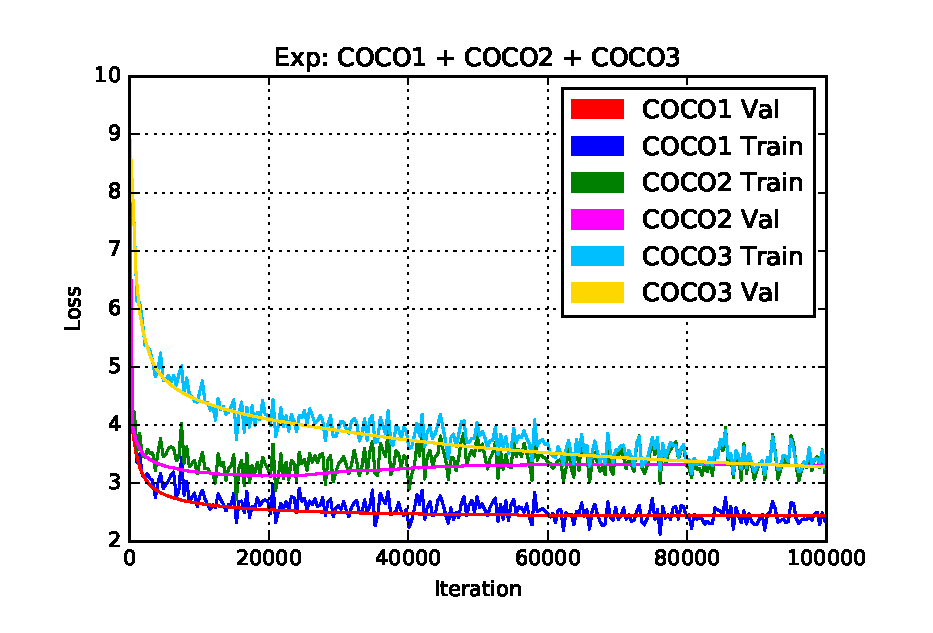
\includegraphics[width=0.8\linewidth]{Chapters/Fig/coco1_coco2_coco3_loss.eps}
  \caption{Training loss during first 10,000 iterations for model with CNN: 16-layer VGGNet, LSTM: 512 hidden states and Adam optimizer}
\end{figure}

\nocite{MLOxford}

Tips and tricks for training neural networks by \cite{DBLP:journals/corr/abs-1206-5533}